\addcontentsline{toc}{section}{\protect\numberline{}ПРИЛОЖЕНИЕ А}
\begin{center}
    \section*{ПРИЛОЖЕНИЕ А}
\end{center}

\subsection*{Настройки тестовой среды}

\label{app:postgresql_conf} % Метка для ссылки
\begin{center}
    \textbf{Файл конфигурации \texttt{postgresql.conf}}
\end{center}
\lstinputlisting[language=,basicstyle=\scriptsize\ttfamily]{code/postgresql.conf}

\newpage


\addcontentsline{toc}{section}{\protect\numberline{}ПРИЛОЖЕНИЕ Б}
\begin{center}
    \section*{ПРИЛОЖЕНИЕ Б}
\end{center}

\begin{table}[H]

\captionsetup{justification=raggedright,singlelinecheck=false}
\caption{Пример таблицы}
\captionsetup{justification=justified,singlelinecheck=false}

\begin{tabular}{|c|c|}
\hline
\textbf{Заголовок} & \textbf{Колонка 3} \\ \hline
Строка 1           & Значение           \\ \hline
Строка 2           & Значение           \\ \hline
\end{tabular}

\end{table}


\newpage


\addcontentsline{toc}{section}{\protect\numberline{}ПРИЛОЖЕНИЕ В}
\begin{center}
    \section*{ПРИЛОЖЕНИЕ В}
    \includegraphics[width=0.5\textwidth]{example-image}
\end{center}


\begin{figure}
\centering
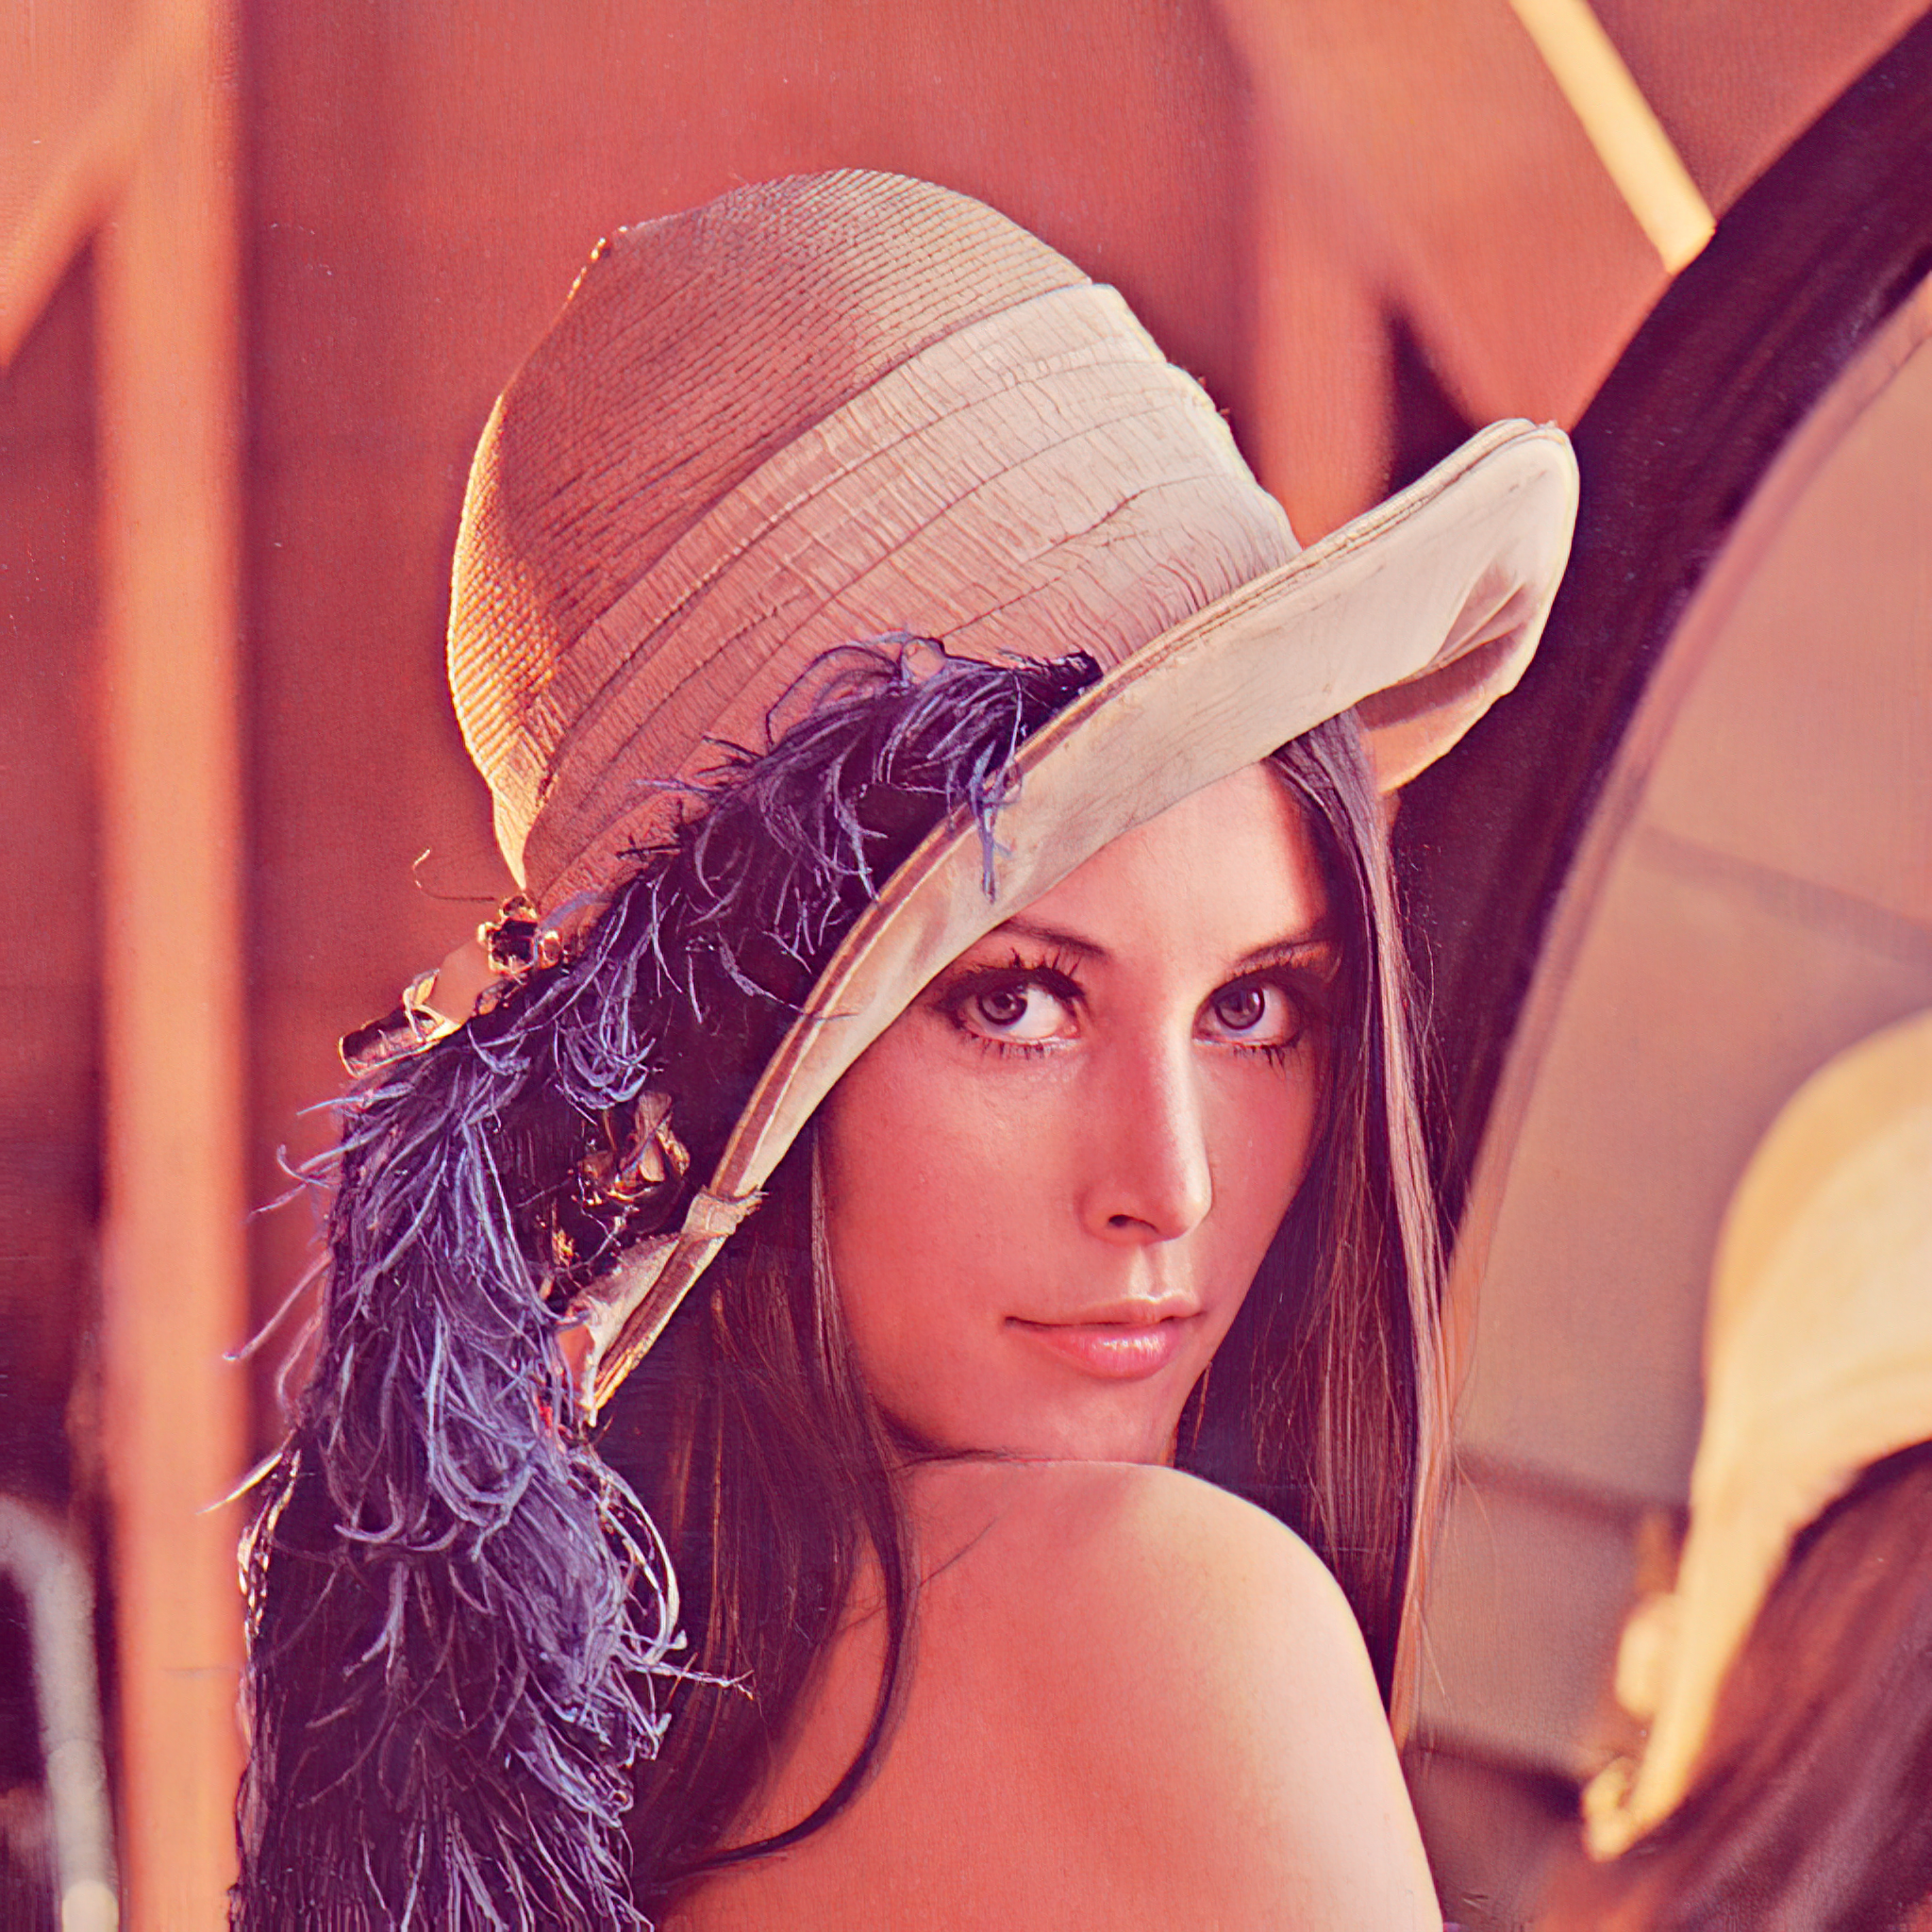
\includegraphics[scale=0.1]{images/lena.png}
\end{figure}

\begin{lstlisting}[language=Java]
public class HelloWorld {
  public static void main(String[] args) {
    System.out.println("Hello, world!");
  }
}
\end{lstlisting}